\label{chap:dense_slam}
\lettrine{C}onsider the following scenario: a robot with a hand-mounted depth sensor scans an unknown scene filled with clutter. The robot's goal is to create a geometric model of the scene that it can use for motion planning and manipulation. If the robot had perfect kinematics, and no uncertainty in its joint angle estimates, creating a geometric map of the scene would be trivial -- it would just involve finding the pose of the sensor at each timestep by looking at the robot's joint encoders, and then stitching together all of the robot's sensor measurements at each pose to create a 3D model. Unfortunately, as we have seen in the previous chapters, many robots do not have perfect joint angle sensing, and some robots have a very large amount of kinematic error. With incorrect joint angle measurments, the model of the scene that the robot creates from its scan will be inaccurate.

\begin{figure}[width=0.5\columnwidth, ht]
	\centering
	\begin{subfigure}{0.5\columnwidth} 
	\centering
	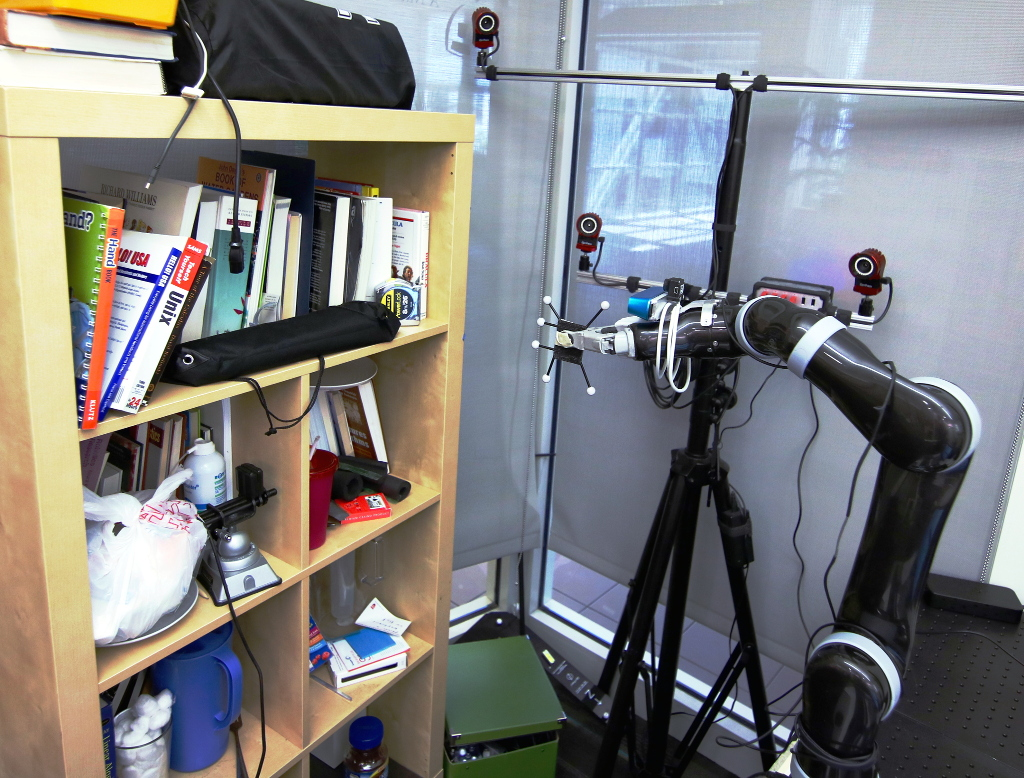
\includegraphics[width=1.0\textwidth]{img/arm_slam/experimental_setup.JPG}
	\caption{Experimental setup.}
	\label{fig:real_robot}
	\end{subfigure}
	 \begin{subfigure}{0.29\columnwidth}
	 \centering 
	 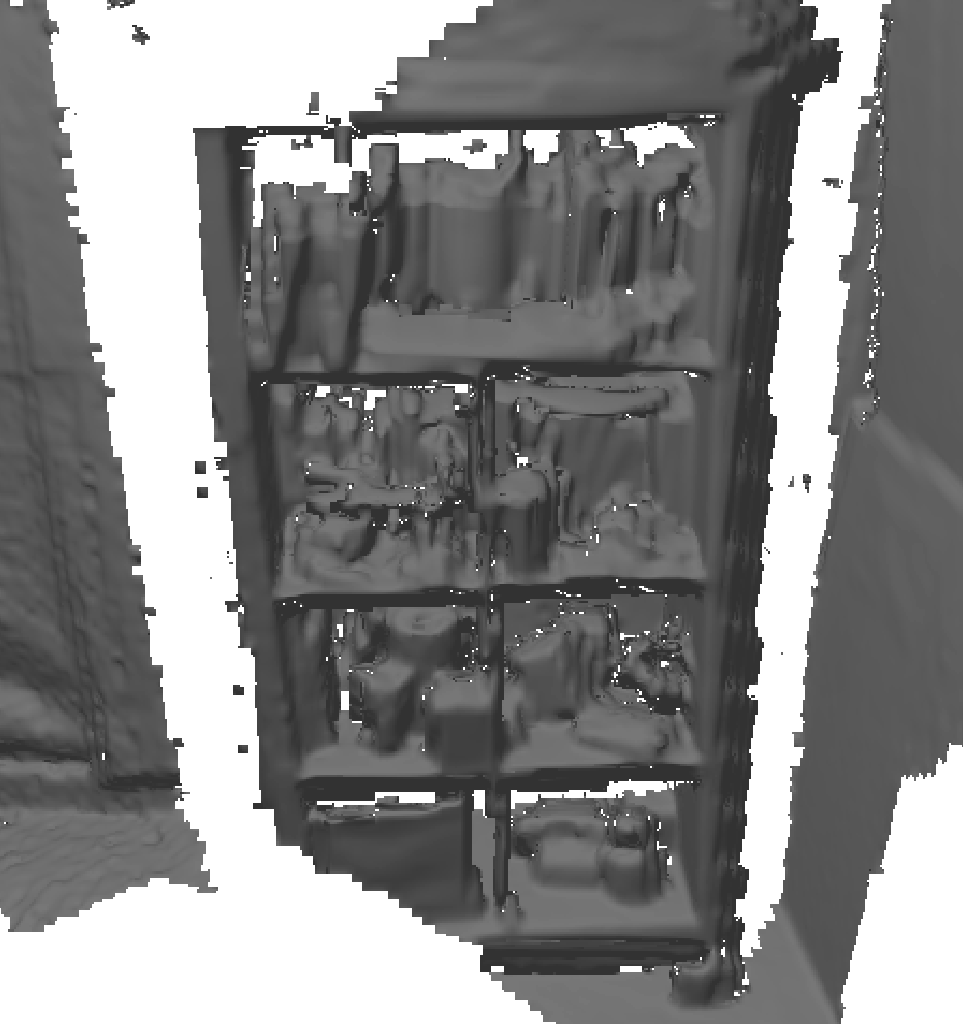
\includegraphics[width=1.0\textwidth]{img/arm_slam/kinfu_bookshelf.png}
	 \caption{Kinect Fusion (baseline).}
	 \end{subfigure}
	\begin{subfigure}{0.29\columnwidth}
	\centering
	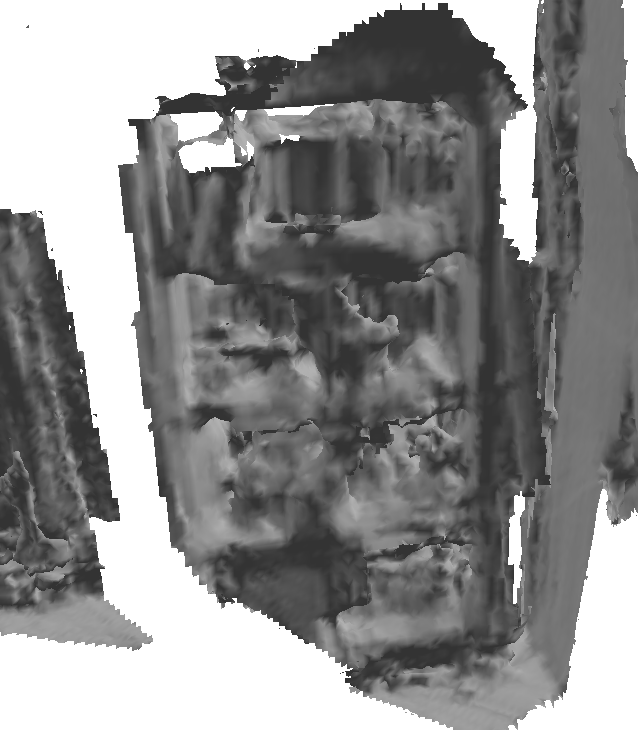
\includegraphics[width=1.0\textwidth]{img/arm_slam/lambert_bookshelf_notrack.png}
	\caption{Forward kinematics. }
	\end{subfigure}
	\begin{subfigure}{0.29\columnwidth}
	\centering 
	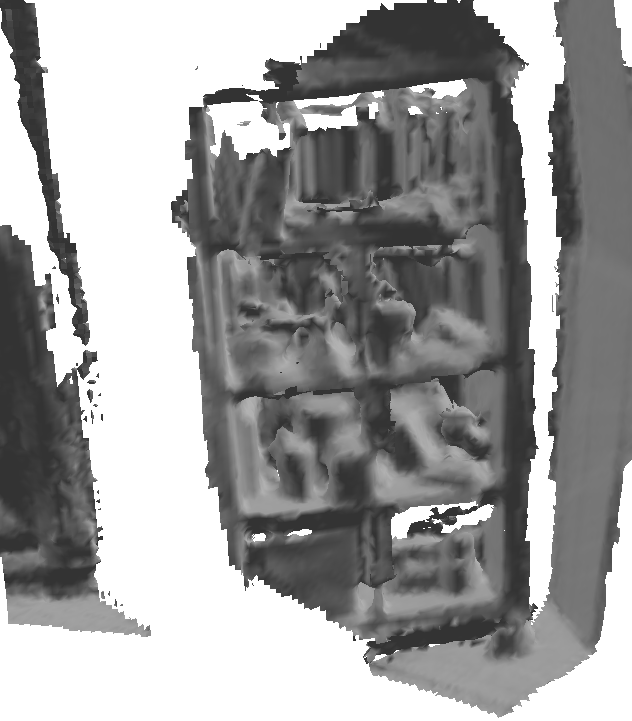
\includegraphics[width=1.0\textwidth]{img/arm_slam/lambert_bookshelf.png}
	\caption{ARM-SLAM}
	\end{subfigure}
	  \begin{subfigure}{0.29\columnwidth}
	 \centering
	 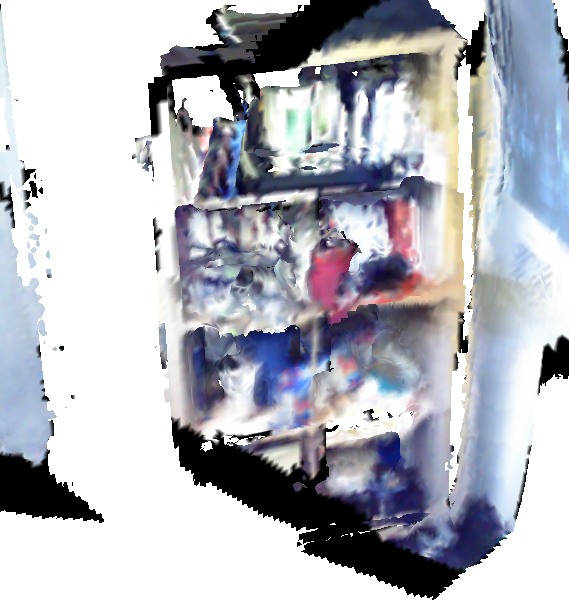
\includegraphics[width=1.0\textwidth]{img/arm_slam/better_bookshelf.png}
	 \caption{Colorized ARM-SLAM.}
	 \end{subfigure} 
	\caption{Robot scans and reconstructions of a bookshelf at 1.5cm resolution using real depth and encoder data (\sref{sec:3d_real}). Our approach (which estimates robot configurations rather than camera poses) results in preservation of fine detail and edges that are lost when only using the robot's forward kinematics, with comparable reconstruction quality to Kinect Fusion.}
	\label{fig:real_reconstructions}
\end{figure}

As we have seen in chapter \ref{chap:dense_external_tracking}, an external depth sensor mounted on a robot's body or affixed somewhere in the scene can be used to correct joint angle error by maximizing the likelihood of a robot's configuration given its sensor data.Can the same approach that we discussed in \ref{chap:dense_external_tracking} be used when the camera is mounted on the robot's hand, and can't see any part of the robot's body? 

Right away, it's clear that we're dealing with a Simultaneous Localization and Mapping (SLAM) problem. The robot's pose at any given time is unknown because of kinematic uncertainty. The model of the world is likewise unknown \apriori. We will therefore have to estimate both the structure of the world and the robot's state simultaneously.

In this chapter, we will explore a dense SLAM technique which simultaneously estimates the robot's joint angles and a dense 3D geometric model of the world \footnote{This chapter is largely restating earlier work found in \cite{Klingensmith2016}}.

\section{Problem Definition}
We have a series of discrete time steps $t = 1, \ldots T$ with synchronized joint encoder measurements $\enc_1, \ldots, \enc_T$ and depth images $\DepthImage_1, \ldots, \DepthImage_T$. The task is to estimate the robot's true configuration $\config_1, \ldots \config_T$ and a geometric model of the scene $\DenseMap$ simultaneously. Formally, we can express this as computing a maximum likelihood estimate of the robot's trajectory and geometric model

\begin{equation}
	\left\{\config_1, \ldots, \config_T, \DenseMap\right\}_{\text{MLE}} = \argmax_{\config_1, \ldots, \config_T, \DenseMap} \Prob\left(\config_1, \ldots, \config_T, \DenseMap | \DepthImage_1, \ldots, \DepthImage_T, \enc_1, \ldots, \enc_T\right)
\end{equation}

\noindent this expression is extaordinarily high-dimensional, and is difficult to directly optimize it, because the dense model $\DenseMap$ correlates every sensor measurement together. Therefore, we solve this problem in the same way as several other dense SLAM techniques (particularly \textit{Kinect Fusion}~\cite{KinectFusion}) by breaking the problem into two parts: first, tracking the sensor with respect to a fixed dense map, and second, updating the dense map with respect to a fixed sensor pose.These two steps, performed rapidly in alteration can be made to simultaneously construct a map and track the pose of the sensor. The trade off is that both the pose and structure of the map can drift over time as small errors accumulate.

\subsection{Mapping the Scene}
Given a set of depth images $\DepthImage_1, \ldots, \DepthImage_T$ taken at known poses $C_1, \ldots, C_T$, we wish to construct a 3D geometric model of the scene $\DenseMap$. This is a well-studied problem in computer vision. We chose the volumetric method of Curless and Levoy \cite{Curless1996} known as Truncated Signed Distance Field (TSDF) mapping. This is the same mapping method used by \textit{Kinect Fusion} \cite{KinectFusion}.

Using this method, the 3D model takes the form of a volumetric signed distance function:

\begin{equation}
	\DenseMap = \Phi(\xvec) : \RThree \to [-\tau, \tau]
\end{equation}

\noindent where $\tau$ is a small radius around the surfaces of objects. The  TSDF maps volumetric points in the scene $\xvec$ to their distance to the nearest surface. Inside objects, the the distance is negative, and outside the distance is positive. Exactly at the surface, the distance is zero. Therefore, the surface of the scene is implicitly represented as the level set $\Phi(\xvec) = 0$.

To generate a TSDF from a series of depth images, we take all the points $\pixel_i \in \DepthImage$ in the point cloud of each depth image, compute its surface normal $\mathbf{n}_i$, and use this to construct a linearization of the distance field near $\pixel_i$. For all of the points $\xvec$ within a radius $\tau$ of $\pixel_i$, we set its signed distance $\Phi(\xvec)$ to the linearized value derived from the surface normal. When the linearizations of several pixels intersect, we merely average the distances. Curless \cite{Curless1996} proved that this method minimizes the squared distance of points in the point cloud to the implicit surface generated by $\Phi$.

In practice, this is accomplished by storing voxels $V$ within a region of interest. Each discrete voxel contains an estimate of the signed distance, and a weight which is used to produce a running average of the TSDF as new measurements accumulate. Algorithm \ref{alg:TSDF} describes how to fuse a new depth image at a known pose into the TSDF.

\begin{algorithm}
\tcp{Given a depth image, sensor pose, previous TSDF, previous voxel weights, a weighting function, a volume of interest, and a truncation distance}
\KwIn{$\DepthImage, C, \Phi^{(t - 1)}, W^{(t - 1)}, w,  V, \tau$}

\tcp{Inverse of the camera transform}
$C' \gets {C}^{-1}$

\tcp{Initialize the new TSDF to the previous one}
$\Phi_{t} \gets \Phi_{t - 1}$

\tcp{Initialize the weights}
$W_{t} \gets W_{t - 1}$

\For{$\mathbf{v} \in V$}
{
    \tcp{Depth of voxel $\mathbf{v}$}
    $\mathbf{v}_c \gets C' \mathbf{v}$
	
	\tcp{Current depth measurement for the voxel.}
	$d_i \gets \DepthImage\left[\Proj(\mathbf{v}_c)\right]$
	
	\tcp{Dist to camera plane.}
	$d_v \gets \mathbf{v}_{c}(z)$
	
	\tcp{Locally linear approximation.}
	$u \gets d_v - d_i$
	
	\tcp{If dist within $\tau$}
	\If{$|u| < \tau$}
	{
	    \tcp{Weighted average}
		$\Phi_{t}(\mathbf{v}) \gets \frac{W_{t}(\mathbf{v}) \Phi_{t}(\mathbf{v}) + w(u) u}{W_{t}(\mathbf{v}) + w(u)}$
		
		$W_{t}(\mathbf{v}) \gets W_t(\mathbf{v}) + w(u)$
	}
}
 
\KwOut{$\Phi_{t}, W_{t}$}
\caption{\textsc{FuseTSDF}}
\label{alg:TSDF}
\end{algorithm}

Using a TSDF to model the scene allows us to average out sensor measurement error as depth images accumulate. The TSDF, since it is continuous and volumetric, also has the advantage of having well-defined gradients $\nabla \Phi$, which are easy to compute using finite differencing.

\subsection{Tracking the Arm}
Assuming a fixed dense map $\DenseMap$, the problem of tracking the arm becomes significantly easier, since we can use the Markov assumption such that the current configuration of the robot is conditionally independent of all the previous configurations, joint encoder measurements and depth images:

\begin{align}
	\config_{\text{MLE}} &= \argmax_{\config} \Prob\left(\config | \DepthImage_T, \enc_T, \DenseMap\right) \\
						 &= \argmax_{\config} \frac{\Prob\left(\DepthImage_T | \config, \DenseMap\right)\Prob\left(\config | \enc_T\right)}{\Prob(\DepthImage_T, \enc_T, \DenseMap)} \\
						 &= \argmax_{\config} \log \Prob(\DepthImage_T | \config, \DenseMap) + \log \Prob(\config | \enc_T)				 
						 \label{eqn:dense_map_track}
\end{align}

\noindent notice that \eqnref{eqn:dense_map_track} bears a striking resemblance to \eqnref{eqn:dense_model_track}, only with an additional term for the dense map $\DenseMap$. This is because with a known map, the problem of tracking the robot arm using a depth image of its own body is exactly equivalent to tracking the robot arm using a depth image of a rigid body attached to its base. In this context, the dense map of the scene can be seen as \textit{just another link} of the robot that is attached rigidly to its base.

With this framework in mind, it is possible to use the same algorithm as in chapter \ref{chap:dense_external_tracking} to track the robot, replacing points on the robot's body with points in the dense map. This is essentially what we do in \cite{Klingensmith2016}, except our representation of the dense map $\DenseMap$ is volumetric, rather than point-based. The joint encoder posterior here is exactly the same as in \eqnref{eqn:dense_model_track}, so we use the same method to compute it.

\subsubsection{Depth Image Posterior}
Assume that the points in the depth image are really samples of points on the surface of $\DenseMap$ that have been corrupted by isotropic Gaussian noise. That is, for each $\pixel_i \in \DepthImage$, assume that there exists a point $\xvec_i~\text{s.t}~ \Phi(\xvec_i) = 0$ that corresponds to a point on the surface of $\DenseMap$, and

\begin{equation}
	\pixel_i \sim \xvec_i + \mathcal{N}(0, \Sigma_\pixel)
\end{equation}

\noindent where $\Sigma_\pixel = \sigma_\pixel \eye$, and $\sigma_\pixel$ is the variance of the depth image noise. If $\pixel_i$ is already very close to $\xvec_i$, then the value of the distance field $|\Phi(\pixel_i)| \approx \|\pixel_i - \xvec_i\|$, and therefore

\begin{equation}
	\Prob\left(\pixel_i | \DenseMap\right) \approx \exp{\frac{-\|\Phi(\pixel_i)\|^2}{2 \sigma_\pixel}}
\end{equation}

Assuming conditional independence among all the pixels in the depth image, we arrive at the expression for the log-likelihood of the depth image posterior from equation \ref{eqn:dense_map_track} as

\begin{align}
	\log \Prob(\DepthImage | \config, \DenseMap) &\approx \log \prod_{\pixel_i \in \DepthImage} \exp{\frac{-\|\Phi(\pixel_i)\|^2}{2 \sigma_\pixel}} \\
				&= -\frac{1}{2 \sigma_\pixel}\sum_{\pixel_i \in \DepthImage}\Phi(\pixel_i)^2 
				\label{eqn:log_likelihood_dense_map}
\end{align}

\noindent note that this is only valid if the pose estimate is already very near the true pose of the sensor. Otherwise, the points from the depth image may be mis-matched to points in the dense map. Depending on the geometry of the scene, the mis-matching could be more or less severe. For instance, if the world consists of a single plane, this method would not be able to distinguish between points on the plane, and all poses that move parallel to the plane will be treated as equally probable (this is a problem that other TSDF methods suffer from as well).

\section{Algorithm Implementation}
As in chapter \ref{chap:dense_external_tracking}, we use stochastic gradient descent of the log-likelihood function to obtain a pose estimate for the robot arm. We interleave this pose estimation step with a TSDF mapping step following \algref{alg:TSDF}. The result is a system which generates a consistent 3D map and corrects the robot's joint angles in real time.

\subsection{TSDF Mapping}
We use the TSDF mapping system from our earlier work \cite{Klingensmith2015}. This mapping system (called \textsc{Chisel}) represents the TSDF as a spatial hash map of voxels. Each voxel stores a 16-bit signed distance, a 16-bit weight, and a 32-bit color (which is not used for tracking). The TSDF grows as more surfaces are observed, but unlike other systems, \textsc{Chisel} stores only voxels that are near surfaces, rather than the entire scene. This allows very large scale maps to be stored efficiently.

\subsection{Stochastic Gradient Descent}
The gradient of the log-likelihood function expressed in \eqnref{eqn:log_likelihood_dense_map} with respect to the robot's configuration $\config$ can be computed as a simple application of the chain rule

\begin{equation}
	\frac{\partial}{\partial \config} \log \Prob(\DepthImage | \config, \DenseMap) = -\frac{1}{2 \sigma_\pixel} \sum_{\pixel_i \in \DepthImage}\Phi(\pixel_i)\J_{\pixel_i}\trans \nabla \Phi(\pixel_i)
\end{equation}


\begin{algorithm}

\tcp{Where $\qvec_e^{(t)}$ are the motor encoders at time $t$,  $\lambda$ is a learning rate, and $\gamma$ is a regularization parameter.}
\KwIn{$\DepthImage_t, \enc_t, \Phi^{(t - 1)}, \lambda, \config^{(t- 1)}$}

$\config^{(k)} \gets \config^{(t - 1)}$

\Repeat{\text{convergence}}
{
	\tcp{The camera transform given the robot's joint angles.}
    $T_{\qvec} \gets F_{\text{cam}}(\qvec^{(k)})$
    
	\tcp{Gradient of the depth image posterior.}
	$\nabla C \gets  \frac{1}{\sigma_\pixel}\sum_{\pixel \in \DepthImage_t} \left[\Phi^{(t - 1)}\left[T_{\qvec} \pixel\right] \mathbf{J}_{\pixel}^T\nabla \Phi^{(t - 1)}\left[T_{\qvec} \pixel\right]\right]$
	
	\tcp{Descend the gradient.}
	$\config^{(k)} \gets \config^{(k)} - \lambda\left(\nabla C  + \frac{1}{\sigma_\config}\left(\qvec - K_\enc(\enc_t)\right)\right)$
}

$\config_t \gets \config^{(k)}$

\tcp{Mapping step.}
$\Phi^{(t)} \gets \textsc{FuseTSDF}\left(\Phi^{(t - 1)}, \DepthImage_t, \configc_t\right)$
 
\KwOut{$\config_t, \Phi^{(t)}$}
\caption{ARM-SLAM}
\label{alg:artfu}
\end{algorithm}

\section{Experiments}
\label{sec:experiments}
 
We conducted three types of experiments to observe the behavior of this algorithm; 2D simulation experiments, 3D simulation experiments, and a real robot experiment. \footnote{\textit{Videos are available at \texttt{http://youtu.be/QrFyaxFUs9w}}}

\subsection{2D Simulation}
\label{sec:2D_sim}
In the simple 2D simulation experiment, a 3-link serial robot manipulator with a simulated 1D depth sensor scans a scene. We added zero-centered Perlin \cite{Perlin02} noise to its joint encoder readings. That is,
 %
\begin{equation}
\enc_t = \config_t + \beta_n\textsc{Perlin}\big(s_n \config_t\big)
\end{equation}

\noindent where $s_n, \beta_n$ are parameters which control noise frequency and magnitude, respectively. In our experiments, $s_n=1.0, \beta_n=0.2$. The simulated depth image is noiseless.

For the world model, we constructed a  simple 2D {TSDF}. We compare the performance of ARM-SLAM (\algref{alg:artfu}) against a simple unconstrained descent algorithm which assumes the sensor can move and rotate freely, without considering the robot kinematics (\figref{fig:2d_experiment}). We found that ARM-SLAM managed to both reduce end effector error and dramatically reduce model error (\tableref{table:2d_experiment_data}), whereas just using a 2D dense fusion technique without constraining using the robot's kinematics resulted in severe, unrecoverable drift because of the scene's self-similarity and the robot's fast motion. Note that in the real experiments, there is comparatively much less actuator noise, and a much smaller scene than in the 2D experiments.

\begin{figure}[ht]
\centering
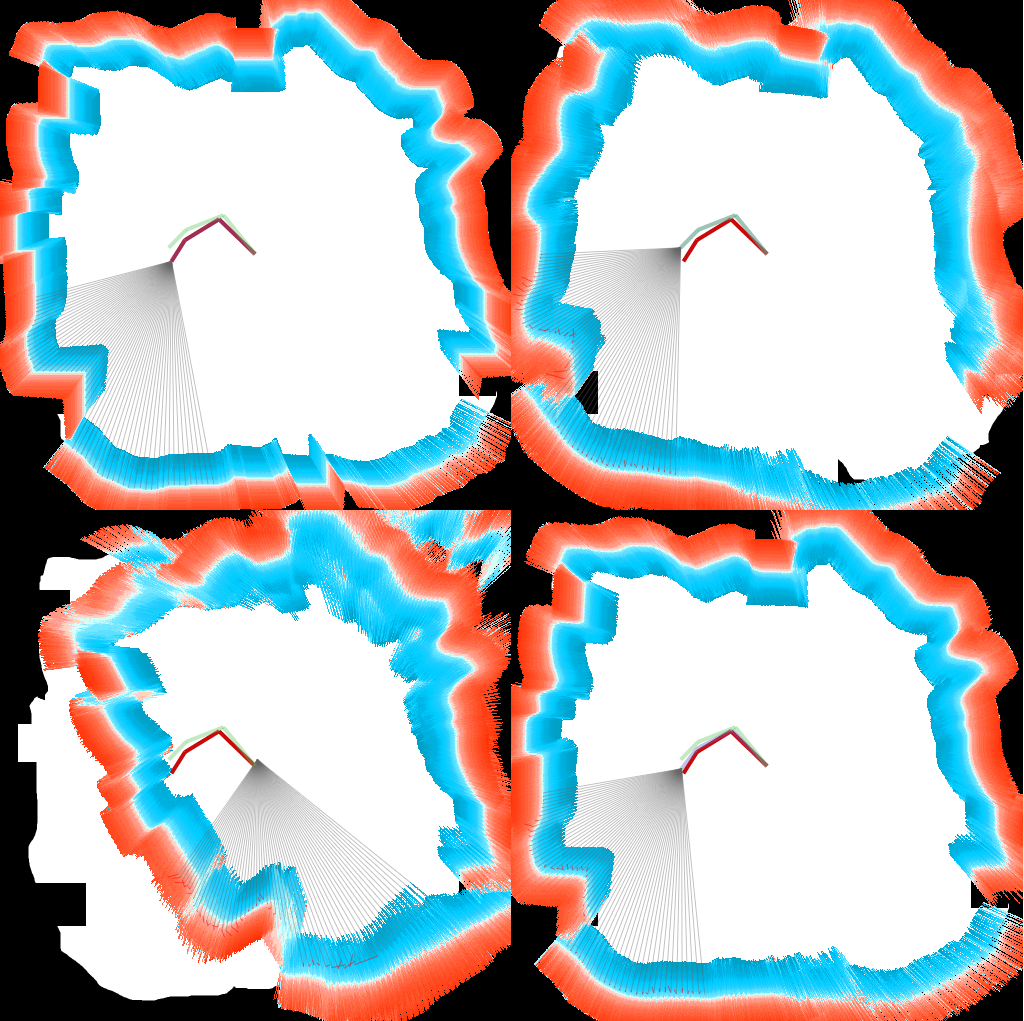
\includegraphics[width=0.78\columnwidth]{img/arm_slam/2d_experiments/2d_end.png}
\caption{2D simulation experiment (\sref{sec:2D_sim}). The robot is shown in red. The simulated depth image is shown as grey rays. The TSDf is shown as orange or blue pixels. Top left shows the ground truth {TSDF}, top right is with forward kinematics only (with actuator uncertainty). Bottom left corrects actuator noise using unconstrained dense fusion. Bottom right corrects using ARM-SLAM.}
\label{fig:2d_experiment}
\end{figure}

\begin{table}
 \begin{tabular}{*5l}
          \hline
             $t$ &      & \textit{Fwd. Kin.}  & \textit{Dense Fusion} & \textit{ARM-SLAM} \\ \hline
             \multirow{4}{*}{500} & EE Err. (pix.)      & $5.2 \pm 5.9$ & $3.4 \pm 4.2$ & $\mathbf{0.8 \pm 0.7}$ \\ 
              & Jnt. Err (rad.)                 & $0.08 \pm 0.06$ & $ - $ & $\mathbf{0.06 \pm 0.05}$ \\
              & SDF Err (pix.)                  & $1.4 \pm 1.7$ & $0.8 \pm 0.8$ & $\mathbf{0.5 \pm 0.3}$ \\ 
              & Class Err (\%)                     & $5.7 \pm 3.2$ & $4.7 \pm 2.3$ & $\mathbf{3.5 \pm 0.6}$ \\ \hline
              
              \multirow{4}{*}{999} & EE Err. (pix.)    & $9.2 \pm 6.7$ & $14.7 \pm 17.8$ & $\mathbf{1.4 \pm 1.9}$ \\ 
              & Jnt. Err (rad.)                   & $0.17 \pm 0.07$ & $ - $ & $\mathbf{0.08 \pm 0.05}$ \\
              & SDF Err. (pix.)                   & $6.1 \pm 5.3$ & $12.2 \pm 22.2$ & $\mathbf{1.2 \pm 0.8}$ \\ 
              & Class Err. (\%)                     & $11.3 \pm 6.2$ & $9.5 \pm 6.1$ & $\mathbf{4.4 \pm 1.1}$ \\
              \hline
    \end{tabular} 
    \caption{Results for the 2D simulation experiments (\sref{sec:2D_sim}). The end effector error in pixels, joint angle error in radians, distance field error in $10^6$ pixels, and occupancy classification error (the proportion of pixels misclassified as containing an obstacle) is shown for forward kinematics, unconstrained dense fusion, and ARM-SLAM for a dataset with 500 and 999 time-steps. Our approach (ARM-SLAM) reduces all three error terms.}
    \label{table:2d_experiment_data}
\end{table}

%\begin{figure}
%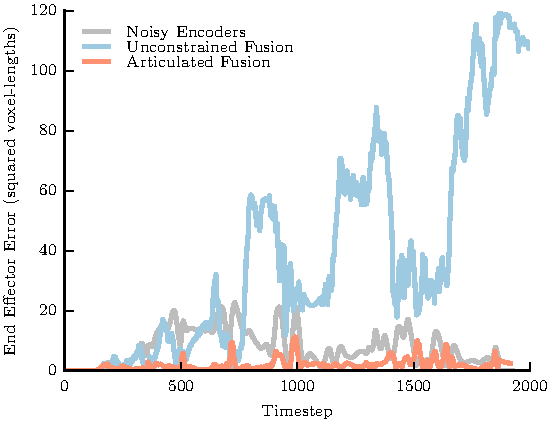
\includegraphics[width=1.0\columnwidth]{img/2d_experiments/ee_error.pdf}
%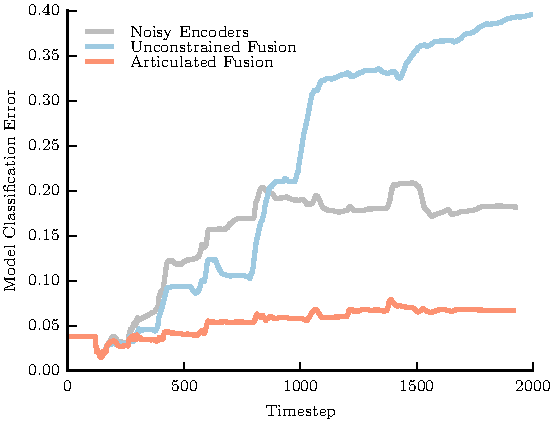
\includegraphics[width=1.0\columnwidth]{img/2d_experiments/class_error.pdf}
%\caption{2D experiment (\sref{sec:2D_sim}) data. Here, end effector error is the squared distance between the reported end %effector position and ground truth. The model classification error is the proportion of \ac{TSDF} voxels that are misclassified (full vs. empty).}
%\label{fig:2d_experiment_data}
%\end{figure}

\subsection{3D Simulation}
\label{sec:3d_sim}

We developed a 3D simulation of a Kinova \textit{Mico} robot with a hand-mounted Occipital \textit{Structure} \cite{StructureSensor} depth sensor. In the simulation, the robot scans a simulated bookshelf. As in the 2D experiments, Perlin noise is added to the ground truth joint angles to simulate actuator uncertainty. We use the \textit{Open Chisel} \cite{Klingensmith2015} chunked {TSDF} library for mapping. The simulated depth image is noiseless. Reconstructions were done at a resolution of 1.5 cm per voxel.

We found that ARM-SLAM was able to correct for very large actuator error (see \figref{fig:3d_experiment_data}), resulting in a final reconstruction near the ground truth (\figref{fig:3d_experiments}). By artificially increasing the actuator noise, we found that ARM-SLAM significantly reduced the end effector error even when the uncertainty in the camera's pose was up to 12 cm (\figref{fig:3d_exp_added_noise}), we also found ARM-SLAM to be more robust to tracking failure from lost data than unconstrained Kinect Fusion (\figref{fig:3d_exp_kinfu}) due to the very strong motion prior from the robot kinematics.

\begin{figure}[ht!]
\centering
\begin{subfigure}{0.4\columnwidth}
	\centering
	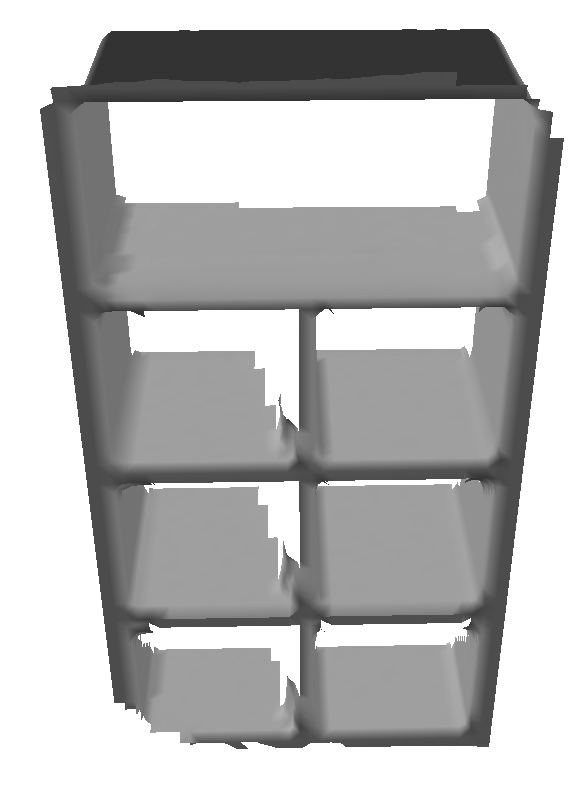
\includegraphics[height=1.0\textwidth]{img/arm_slam/groundtruth_sim.png}
	\caption{Ground truth}
\end{subfigure}
\begin{subfigure}{0.4\columnwidth}
	\centering
	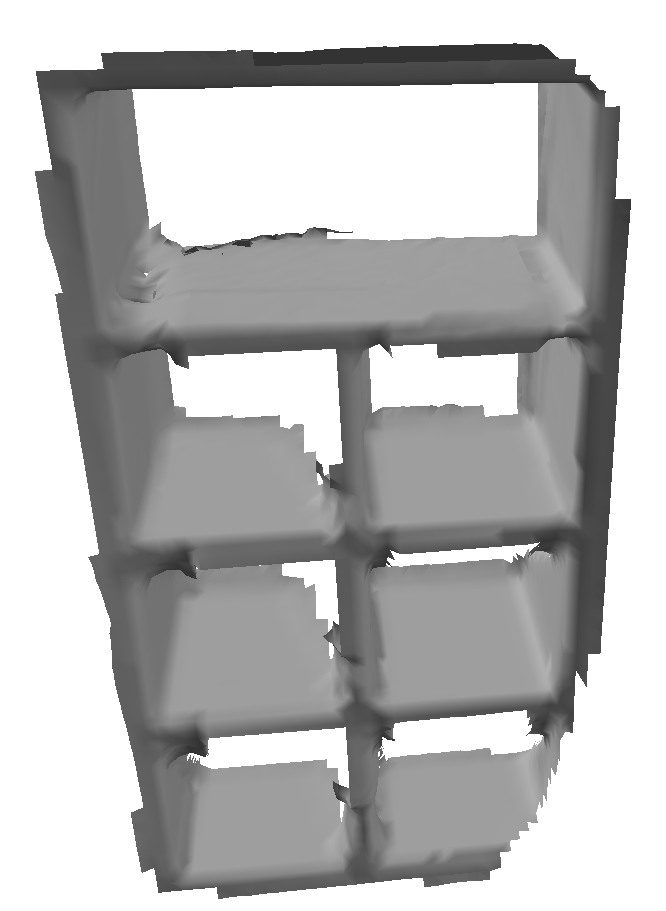
\includegraphics[height=1.0\textwidth]{img/arm_slam/artfu_sim.png}
	\caption{ARM-SLAM}
\end{subfigure}
\begin{subfigure}{0.4\columnwidth}
	\centering
	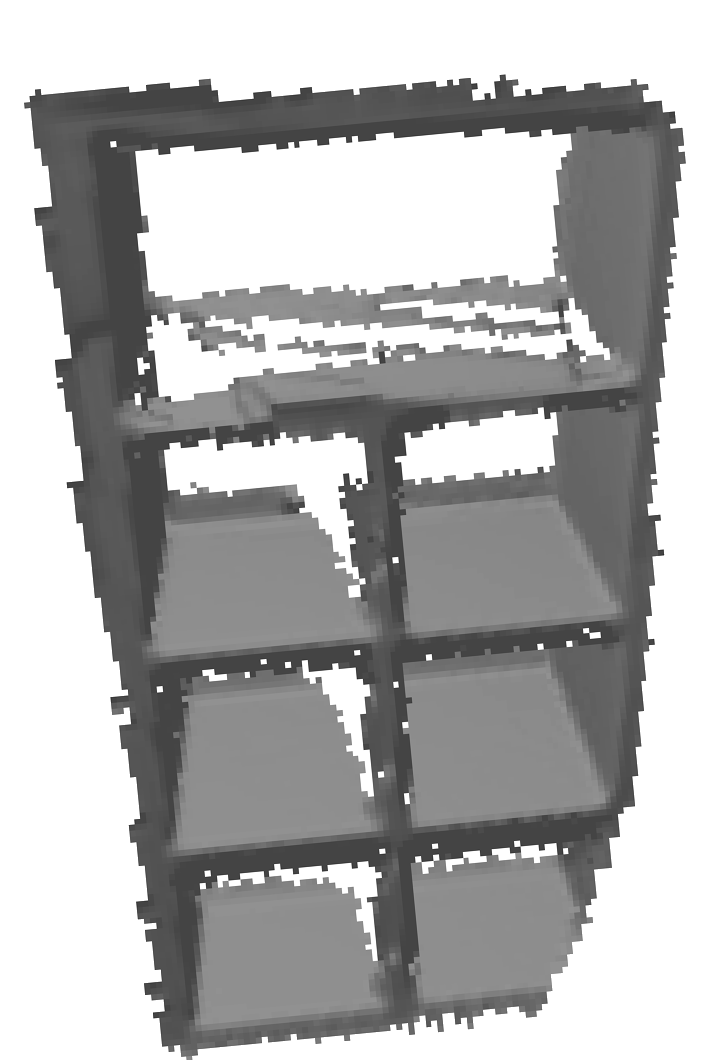
\includegraphics[height=1.0\textwidth]{img/arm_slam/kinfu_sim.png}
	\caption{Kinect Fusion}
\end{subfigure}
\begin{subfigure}{0.4\columnwidth}
	\centering
	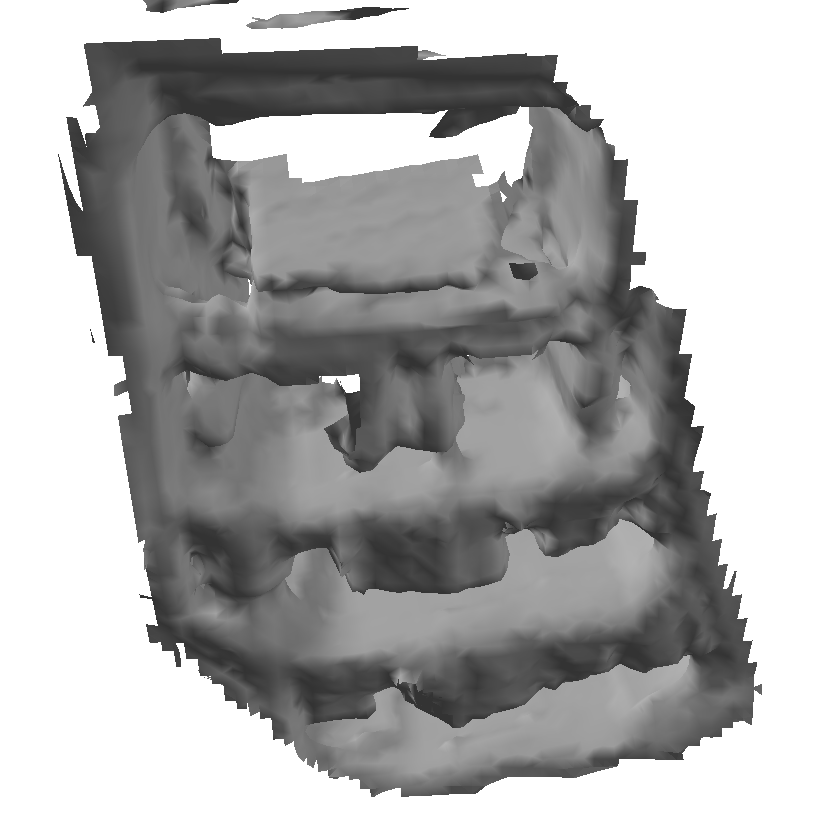
\includegraphics[height=1.0\textwidth]{img/arm_slam/kinematics_sim.png}
	\caption{Forward kinematics}
\end{subfigure}
\caption{Results of the 3D simulation (\sref{sec:3d_sim}) with up to 0.8 radians of added noise per joint.}
\label{fig:3d_experiments}
\end{figure}

\begin{figure}[ht]
\begin{subfigure}{0.5\columnwidth}
	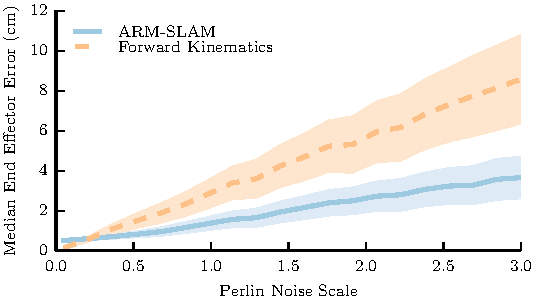
\includegraphics[width=1.0\columnwidth]{img/arm_slam/added_noise.pdf} 
	\caption{3D simulation with added noise.}
	\label{fig:3d_exp_added_noise}
\end{subfigure}
\begin{subfigure}{0.5\columnwidth}
	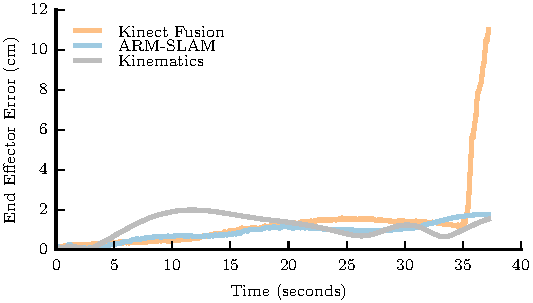
\includegraphics[width=1.0\columnwidth]{img/arm_slam/3d_kinfu_error.pdf} 
	\caption{3D simulation with lost tracking.}
	\label{fig:3d_exp_kinfu}
\end{subfigure} 
\begin{subfigure}{0.5\columnwidth}
	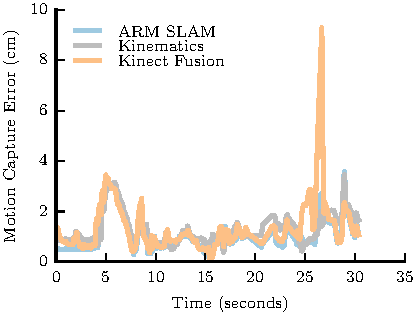
\includegraphics[width=1.0\columnwidth]{img/arm_slam/motion_track.pdf} 
	\caption{Real data validated with motion capture.}
	\label{fig:motion_track} 
\end{subfigure} 
\caption{End effector error observed in the 3D simulation (\sref{sec:3d_sim}) experiments. \figref{fig:3d_exp_added_noise}: 100 trials with different noise seeds are run with increasing noise magnitude. Each trial lasts 60 seconds. The median deviation of the end effector from ground truth is recorded. \figref{fig:3d_exp_kinfu}: in a different simulation, the robot briefly looks away from the scene and then looks back. Kinect Fusion loses tracking. \figref{fig:motion_track}: end-effector deviation in the real dataset as measured by an optical motion capture system, Kinect Fusion briefly loses and then regains tracking.}
\label{fig:3d_experiment_data} 
\end{figure}

\subsection{Bookshelf Scanning}
\label{sec:3d_real}

Using the same framework as in the 3D simulation, we reconstructed a bookshelf with a Kinova \textit{Mico} robot with a hand-mounted Occipital \textit{Structure} sensor (\figref{fig:real_reconstructions}). The robot was teleoperated using a joystick. Beforehand, the Structure sensor was extrinsically calibrated to the robot's hand using the Tsai\cite{Gupta11cameracalibration} method and a fiducial, though extrinsic calibration error cannot be ruled out. The end effector deviation was measured using an \textit{Optitrack} motion tracking system. One challenge of working with the real robot data is that the joint encoders and depth sensor are not synchronized. The joint encoder data is emitted at $\sim 500~\text{Hz}$, whereas the camera data is produced at $30~\text{Hz}$. To compensate for this, we store the robot's configuration space trajectory as a series of linearly interpolated, timestamped waypoints. Using this, we can infer the joint encoder readings at the time when the depth image was received. 

The 3D reconstructions (\figref{fig:real_reconstructions}) show that our method is able to recover 3D structure in the scene that is lost when only the (noisy) forward kinematics are used. This is especially apparent around the edges of the bookshelf and its adjacent walls. Our reconstructions are comparable to Kinect Fusion run at the same voxel resolution (1.5 cm). We measured end-effector motion with an optical 
motion capture system (\figref{fig:motion_track}) and found that Kinect fusion occasionally lost (and regained) tracking due to self-similar surfaces in the bookshelf and surrounding walls. Because of the strong motion prior from the robot's joints ARM-SLAM did not have this issue. However, our data from the motion capture system is too noisy to conclude ARM-SLAM performed any better than forward kinematics at reporting the true pose of the end effector (ARM-SLAM had an end effector deviation of $1.2 \pm 0.9 \text{cm}$ while forward kinematics had a deviation of $1.4 \pm 1.0 \text{cm}$). It may be that extrinsic calibration error between the sensor and rigid hand mount is dominating any error produced at the robot's joints.

\section{Discussion and Limitations}
In this chapter, we introduced a framework (called ARM-SLAM) for dense visual SLAM in a robot's configuration space. We have shown that our approach is capable of reconstructing scenes and reducing actuator uncertainty simultaneously. Unfortunately, ARM-SLAM has several limitations which must be addressed in the next few chapters.

First, since it is a pure model-based dense SLAM approach (like \textit{Kinect Fusion}\cite{KinectFusion}), it suffers from many of the problems that plague these approaches. The system requires clear geometric structure and a large field of view to localize correctly, and since it uses no global \textit{pose graph}, it is susceptible to drift over longer trajectories. Further, we are only able to track the configuration of the robot when a depth image is available. Also like those approaches, the underlying tracking and mapping techniques are largely based on geometric arguments, making it difficult to incorporate probabilistic models. As a consequence, we don't have a way of tracking the uncertainty in the predicted joint angles.

By committing to localization in the configuration space of the robot, rather than $SE(3)$, we gain the benefit of only predicting physically plausible camera poses. We are also able to express costs and priors (such as joint limit and self-collision costs) on robot configuration trivially. On the other hand, error that can't be expressed in the configuration space (such as error in the extrinsic calibration, or motion of the robot base) cannot be corrected for using our technique. Also, the more joints a robot has in comparison to $SE(3)$, the more work our technique has to do to compute Jacobian terms, and the larger the camera motion null-space is (worsening susceptibility to local minima). For instance, a 2-jointed robot pan-tilt head would be comparatively easy to localize vs. a highly redundant 50-jointed snake robot. 

In spite of these limitations, our approach provides a good baseline for more complex SLAM techniques designed to address these problems that we will examine in the next chapter.